\documentclass[main.tex]{subfiles}

\begin{document}

\chapter{Previous work}

\section{Traditional approches to segmentation}
\subsection{Intensity based}


In this approach the underlying assumption is that cells have different intensities than the background, either globally then we apply a fixed threshold on the whole image from the histogram typically using an adaptive threshold method like the Otsu~\cite{Otsu1979} threshold, or maybe locally because of different phenomenons, in which case we use a threshold based on a neighborhood. But in practice this assumption is often violated making these approach not very reliable~\cite{Bengtsson2004}, although it's maybe still used as baseline, or as a starting point for further processing e.g, by morphological filters. \\

\begin{figure}[H]
    \centering
    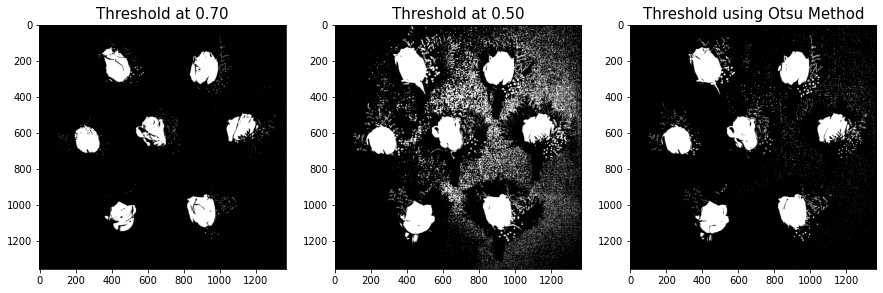
\includegraphics[width=12cm]{images/otsu.png}
    \caption{Otsu threshold compared to manual threshold}
    \label{fig:otsu}
\end{figure}

\subsection{Morphological filters} 
Morphological filters~\cite{Maragos1986, Breen2000} refer to a group of image processing operations that work with images based on shapes. Morphological operations rely only on the relative ordering of pixel values, not on their numerical values. A structuring element is used which corresponds to a shape that slides on the entire image and gets compared with the neighborhood of pixels of all possible, it works differently with each type of operator. A fine distinction is made between binary morphology, and grayscale morphology, where the first is commonly used as a post-processing step, while the latter is used a preprocessing. The fundamental operators are :
\begin{itemize}
    \item Erosion: removes small-scale details from a binary image and reduces the size of regions of interest
    \item Dilation: adds a layer of pixels to both the inner and outer boundaries of regions
    \item Opening: opens up a gap between objects connected by a thin bridge of pixels
    \item Closing: fill holes in the regions while keeping the initial region sizes
\end{itemize}
The combination of these operators creates further more operators such as (top hat, ultimate erosion, alternating filters, skeletonization, connected component transform, morphological gradient ...)~\cite{Maragos1986, Breen2000}. This non linear filters can be very useful in many cases e.g. noise removal, boundary detection, contrast enhancement, shape detection. 

\subsection{Watershed}
Watershed is a very popular region growing method. It considers that every image can be viewed as a topographical surface. It relies not on neighborhood (like classical region growing methods) but rather on intensities (which correspond to the elevation in the image landscape). If we flood this landscape and prevent regions from merging, we obtain a segmentation ~\cite{Bengtsson2004}. Preferably, we construct an energy function whose minimas correspond roughly to regions, typically use the gradient image or distance transform. One major problem with this approach is that it tends to oversegment the image, many solutions were proposed, notably the Seeded watershed approach which restricts the flooding process to flow only from seeded regions, or the use of region merging criteria. Unfortunately, this method still requires extensive user interaction.

\begin{figure}[H]
    \centering
    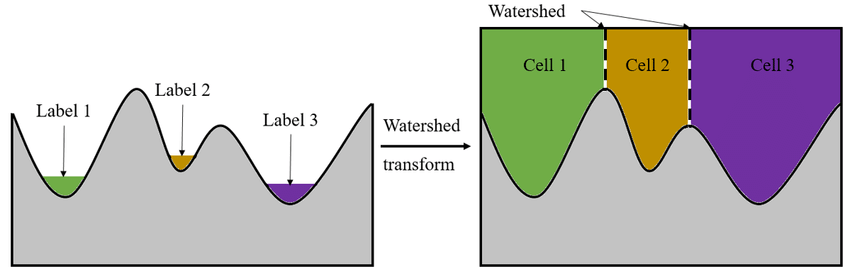
\includegraphics[width=12cm]{images/watershed.png}
    \caption{Example of the pipeline used for watershed segmentation}
    \label{fig:watershed}
\end{figure}
\subsection{Active contour}

Active contour is a type of segmentation technique which can be defined as a deformable model that uses energy forces and constraints to iteratively converge a contour to the boundaries of the desired object's for further processing and analysis. The main application of active contours in image processing is to define smooth shape in the image and forms closed contour for the region. Commonly used active contour models : models involve snake model, gradient vector flow snake model, balloon model and geometric or geodesic contours~\cite{Bengtsson2004}.

\begin{figure}[H]
    \centering
    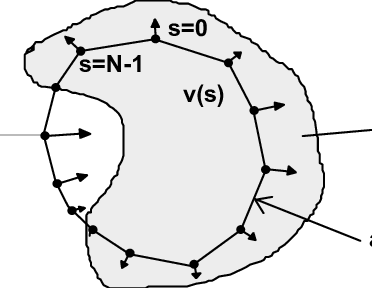
\includegraphics[width=4cm]{images/ac.png}
    \caption{Example of the Active contour}
    \label{fig:ac}
\end{figure}

The energy function of the active contour model is given by the sum of its external energy and internal energy
\begin{equation}
    E_{\mathit{snake}} = \int_{0}^{1} (E_{\mathit{internal}}(v(s)) + E_{\mathit{image}}(v(s))) + E_{\mathit{constraint}}(v(s)))\quad ds
\end{equation}
\paragraph{B-Spline Snakes} In ~\cite{Brigger2000}, the author proposed a novel B-spline formulation to the Snake model, which reduces the number of control points required and removing the internal energy term, the smoothness of the curve is only addressed implicitly thought knots spacing.

\paragraph{Hermite Snake with control tangent} In ~\cite{Uhlmann2016}, the authors formulate a different Spline interpolated Snake using Hermite-spline interpolation. This approach distinguishes itself from other spline formulations by its ability to generate corners easily using tangent control, where previous method used to use more control points to approximate corners, and were very inefficient. They reformulate the energy function as follows for a Snake S parametrized by $r \in [0;1]$:

\begin{equation}
    E_{\mathit{directional}} = -\frac{1}{L} \int_{S}\left| \left< \theta, \frac{r^{'}}{||r^{'}||}\right>\right| \rho(r) \quad dr
\end{equation}
where $\theta$ is the gradient orientations, $\rho$ is the gradient magnitude. r, and r' correspond to the position and the derivative of the curve respectively.\\

The resulting snake energy tend to place the snake contour in regions of high gradient amplitude  and to align its tangent vectors with the local orientation of the gradient.

\begin{figure}[H]
    \centering
    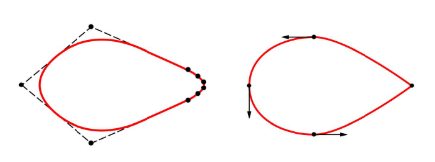
\includegraphics[width=8cm]{images/hermite.PNG}
    \caption{Hermite spline with tangent control}
    \label{fig:ac}
\end{figure}


% \paragrpah{Gas of circles model} In ~\cite{Molnar2016}, the authors present an active contour model that can detect cell nuclei and their morphology in high density cultures with many overlapping cell nuclei. We combine the “gas of near circles” active contour model, which favors circular shapes but allows slight variations around them, with a new data model. This captures a common property of many microscopic imaging techniques: the intensities from superposed nuclei are additive
\section{Deep learning approaches}
\subsection{Bottom up (Proposal free)}
In proposal free (Bottom up) Approaches, first a pixel labeling is made, followed by a clustering step.
\subsubsection{UNet}
Unet is a fully convolutional neural network made for the purpose of semantic segmentation. From \textbf{Figure \ref{fig:unet}} we can see the architecture diagram looking like a U shape, hence it's name Unet. The basic idea of the UNet is to first obtain a lower-dimensional representation of the image through a traditional convolutional neural network, and then upsamples that low-dimensional representation to produce the final output segmentation map (previous methods used to directly upsample the feature maps of the last layer using pixel interpolation, but found that they could just build a decoder networks that gradually upsamples the features which obtained significant better results). Unet uses skip connections to escape the vanishing gradient, as well as identity learning. In order to achieve instance segmentation with unet different approaches have been used, either by applying a threshold on the probabilities, or using binary opening morphological filters, or by using a Constrained Random Field.

\begin{figure}
    \centering
    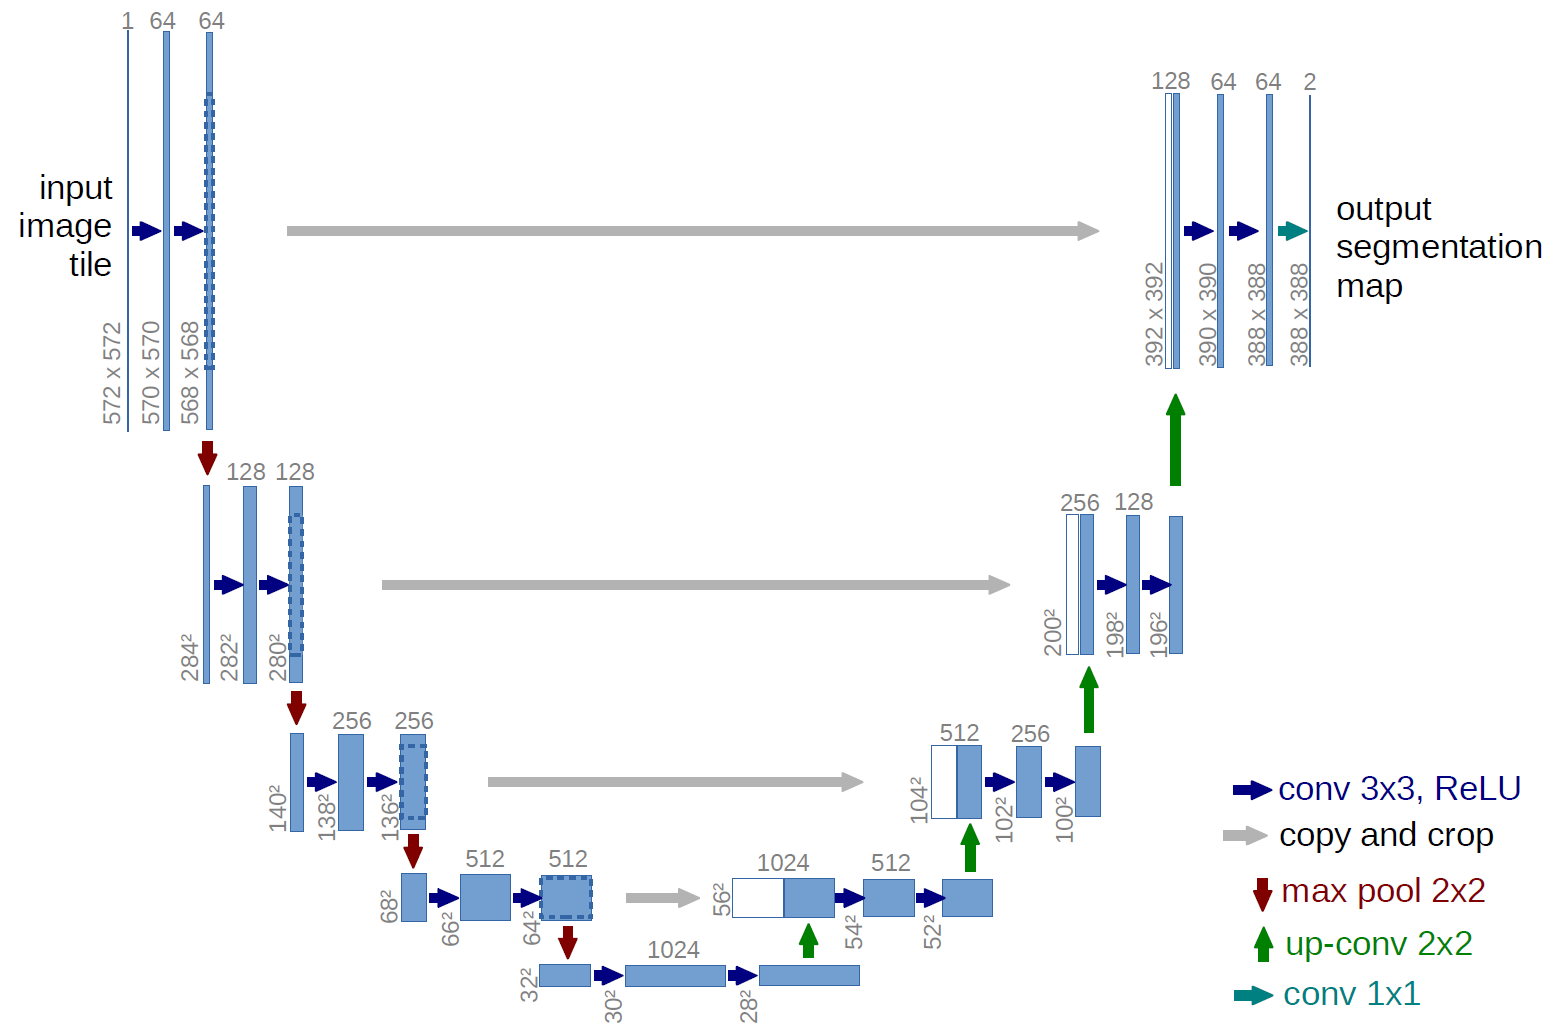
\includegraphics[width=10cm]{images/unet.png}
    \caption{Unet architecture}
    \label{fig:unet}
\end{figure}

\paragraph{Two class Unet} Typically when classifying cells, we would like to separate a foreground from the background as done by ~\cite{Ronneberger2015}. Then pixels are grouped into connected components after running a threshold $\sigma$ 
\paragraph{Three class Unet} An improvement of two class Unet, is simply incorporating a third class corresponding to borders like in ~\cite{Caicedo2019}. This method tend to have higher precision than it's two class variant.

\paragraph{Swin UNet}~\cite{Cao2021} Despite the remarkable performance of CNN, they are still unable to learn global and long-range semantic information and interaction due to the localization of the convolution operation. Swin-Unet is a Unet-like pure Transformer for medical image segmentation, as shown in \textbf{Figure \ref{fig:swin}}. It creates tokenized image patches, which then are fed into the Transformer-based U-shaped Encoder-Decoder architecture with skip-connections and internally use self attention mechanicsm. The obtained results surpass the state of the art convolutional. We can swap previous encoders with swin-unet. Although this model requires a pretraining.

\begin{figure}
    \centering
    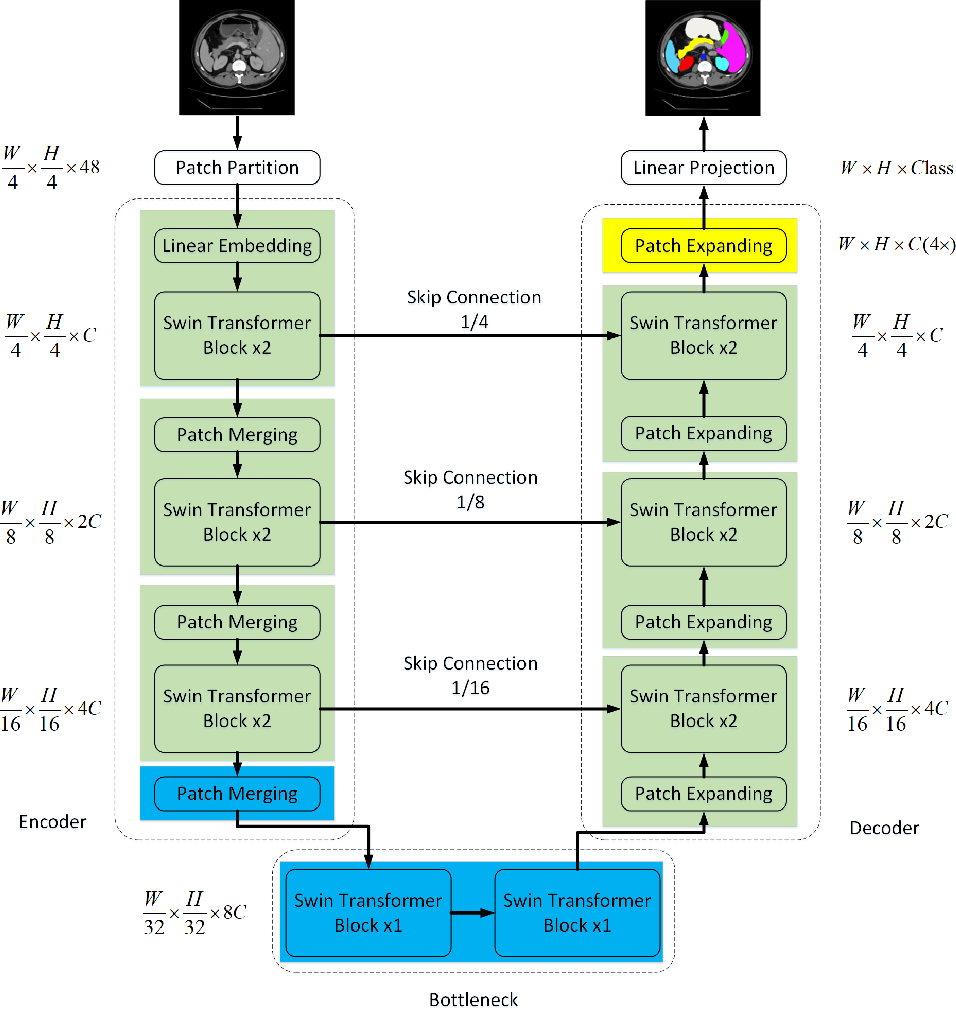
\includegraphics[width=10cm]{images/swin.png}
    \caption{Swin Unet : a pure transformer unet architecture for semantic segmentation}
    \label{fig:swin}
\end{figure}

\paragraph{Deep watershed}In ~\cite{Bai2016}, the authors use a neural network to learn the energy of the watershed transform, in which each basin corresponds to a single occurrence and all ridges in the energy domain are at the same height. As a result, the watershed cut corresponds to a single threshold in energy, which prevents excessive segmentation. The modules introduced can be applied to any segmentation backbone, as the only input given is the RGB image with it's semantic segmentation as shown in the \textbf{Figure \ref{fig:deepwatershed}}.

The approach uses a two step network: 
\begin{itemize}
    \item Direction  network
    \item Watershed Transform network
\end{itemize}

\begin{figure}[H]
    \centering
    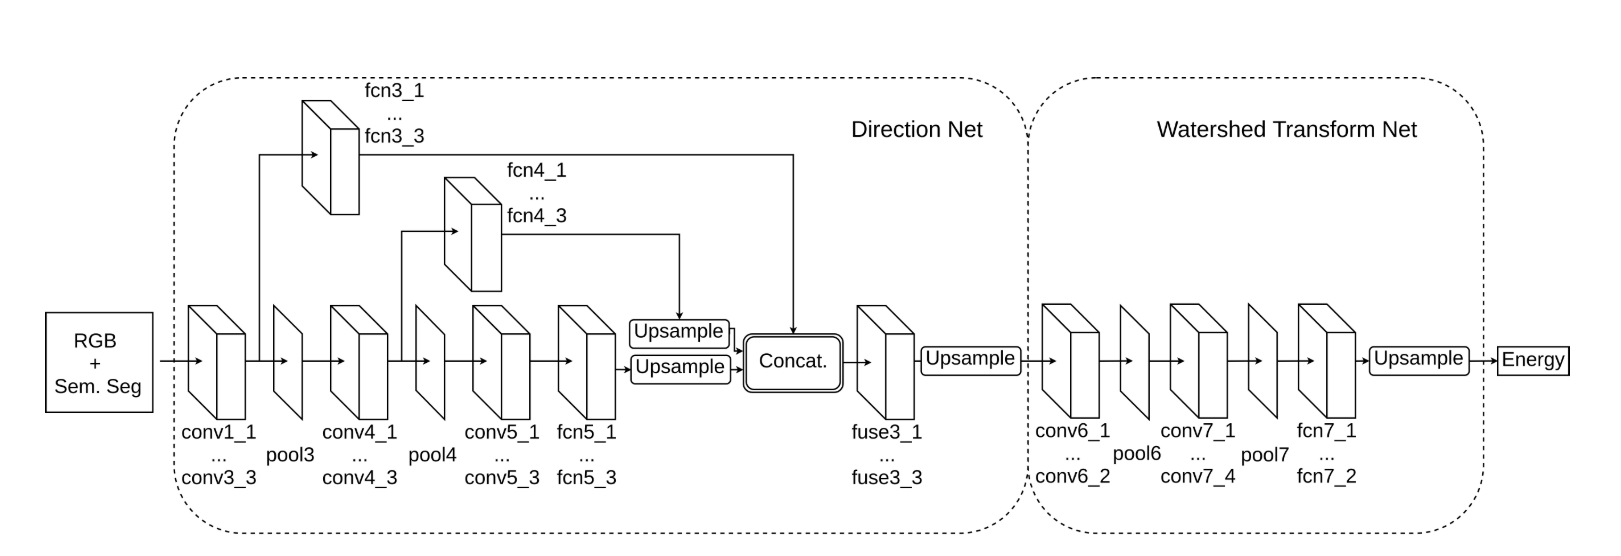
\includegraphics[width=16cm]{images/deepwatershed.png}
    \caption{Deep watershed architecture}
    \label{fig:deepwatershed}
\end{figure}



\subsection{Top down (with proposal)}
\subsubsection{Mask RCNN}
In ~\cite{he2017mask}, the authors present Mask R-CNN, a relatively simple and flexible model that performs instance segmentation by object detection with simultaneous generation of high-quality masks. Mask R-CNN builds up from the Faster R-CNN approach. It replaces the imprecise ROI pooling layer with a new layer called ROI align which allows the construction of very accurate segmentation masks, and adds an object mask prediction branch in parallel as an improvement (see \textbf{Figure \ref{fig:maskrcnn}}). Mask-RCNN is built on a backbone convolutional neural network architecture for feature extraction that can be any convolutional neural network designed for images analysis, such as ResNet-50. In ~\cite{johnson2018adapting} proposed an adaptation to the case of cell segmentation.

\begin{figure}[H]
    \centering
    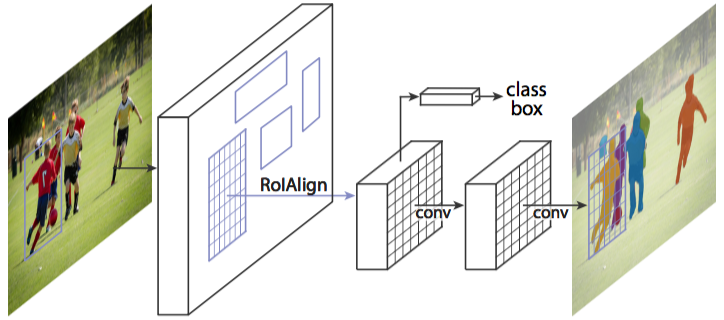
\includegraphics[width=10cm]{images/mask-rcnn.png}
    \caption{Mask RCNN architecture}
    \label{fig:maskrcnn}
\end{figure}
\subsubsection{SoloV2}In ~\cite{Wang2020}, the authors propose a new instance segmentation method called SoloV2 (see \textbf{Figure \ref{fig:solo}}) that directly predicts masks for each instance in the image without resorting to bounding box detection suing mask kernel prediction. This method achieved state-of-the-art  results surpassing Mask RCNN both in precision and speed as it can run in real time on consumer grade GPUs.

\begin{figure}[H]
    \centering
    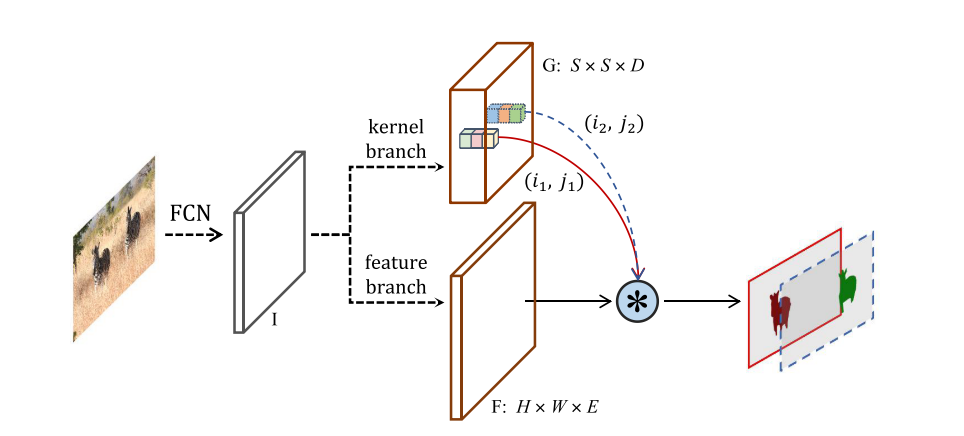
\includegraphics[width=12cm]{images/solov2.PNG}
    \caption{Solov2 architecture}
    \label{fig:solo}
\end{figure}
% \subsection{Region proposal}
% \subsection{Shape refinement}

\subsection{Weak supervised segmentation} One of the problems of cell segmentation in deep learning is that a lot of fully annotated data is needed. Datasets containing hundreds of thousands of fully segmented cells are rare. So typically we would like to relax that constraint and use weaker annotations like positions of cells rather than their full mask per pixel. In ~\cite{Nishimura2019}, the author present a method that does exactly that, they first train a Unet model to localize cells using the provided position annotations. Then, using a back propagation algorithm on each peak of the resulting locations, will show the pixels in the image responsible for the activation of that particular peak. These pixels are then fed into a segmentation (foreground background) using a graph cut algorithm, resulting in a full instance segmentation (see \textbf{Figure \ref{weak}}).
\begin{figure}
    \centering
    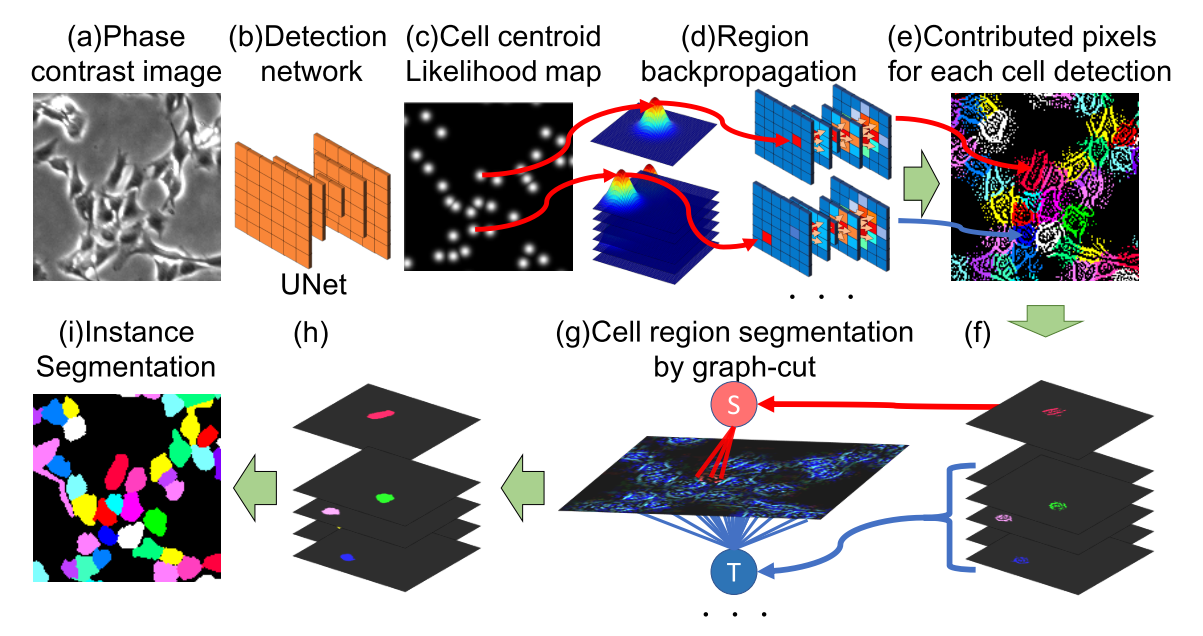
\includegraphics[width=16cm]{images/weak.png}
    \caption{Weak supervised instance segmentation}
    \label{fig:weak}
\end{figure}


\subsection{Recurrent UNet}
In ~\cite{Salvador2017}, the authors reformulate the problem of instance segmentation as a problem of sequential prediction of masks one at a time without requiring further post-processing such as Non maximum suppression. They combine the well established Unet architecture with temporal models LSTM (see \textbf{Figure \ref{fig:cnnlstm}}). the models output one mask at a time until a stop token is output by the model. This approaches uses multitask loss that combines Segmentation Loss(Soft intersection over union)
Classification Loss(Categorical cross entropy loss), Detection Loss(Mean squared error), and a Stop loss.

\begin{figure}[H]
    \centering
    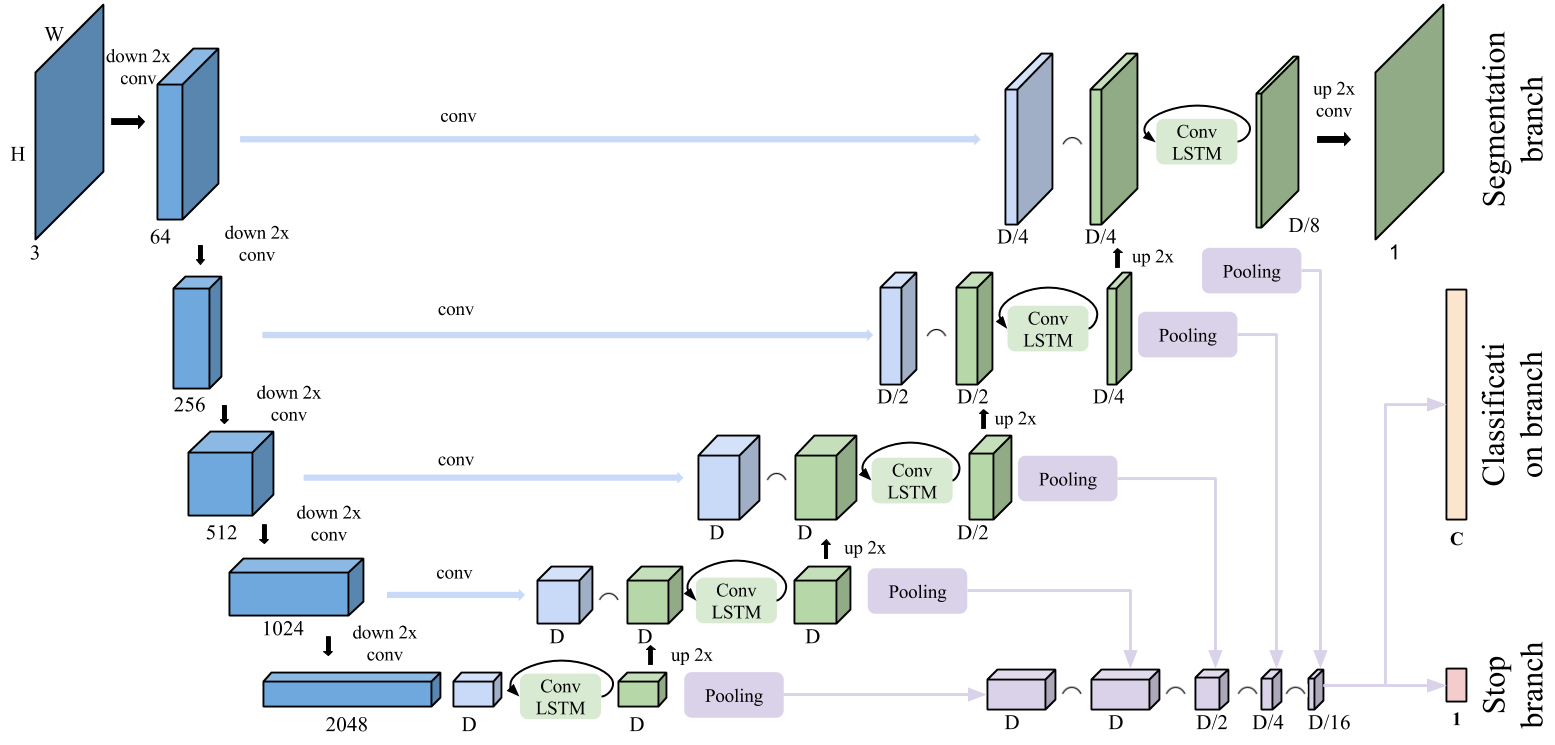
\includegraphics[width=16cm]{images/unetlstm.png}
    \caption{UNet LSTM model}
    \label{fig:cnnlstm}
\end{figure}


\subsection{CellPose} A novel, promising approach called cellpose ~\cite{Stringer2020} aims at solving cell segmentation for all modalities at once with a single model trained on any available images of cells. Their approach consists at predicting gradient flows using a Unet, which will later serve at assigning a sink (a cell identity) to each pixel by following the gradient flow. results shown by the authors are superior to those of StarDist, and Mask RCNN and can model Very complex shapes in different scenarios.

\begin{figure}[H]
    \centering
    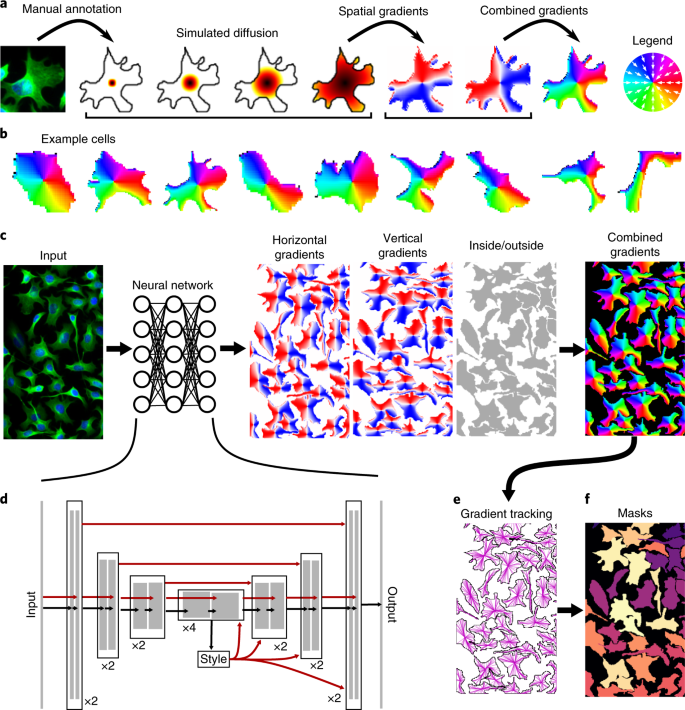
\includegraphics[width=14cm]{images/cellpose.png}
    \caption{Cellpose approach}
    \label{fig:ac}
\end{figure}

\section{Parametric object proposal}
This category of models densely predict parametric objects for all the image and make use of the non maximum operation to keep the highest probable objects. 

\subsection{StarDist}
In ~\cite{Schmidt2018}, the authors propose a novel proposal based approach to instance segmentation using star-convex polygons since they are a far better shape representation than bounding boxes used by previous methods and hence do not require shape refining. They train a convolutional neural network that predicts a polygon for each pixel based on the cell instance at that location. To do so, the binary ground truth masks has to be transformed. for each object, compute the distance transform (which will serve as object probability in order to favor pixels near the center of objects), and a set of M radial distances corresponding to the distances to the boundary of the object by following a radial direction.(see \textbf{Figure \ref{fig:stardistangles}, \ref{fig:radial}}) 

\begin{figure}[H]
    \centering
    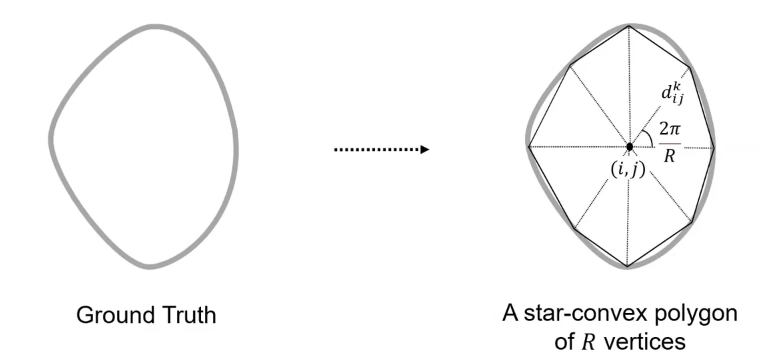
\includegraphics[width=10cm]{images/stardistCreateAnnot.PNG}
    \caption{Creation of the equally spaces angles for Stardist}
    \label{fig:stardistangles}
\end{figure}

\begin{figure}[H]
    \centering  
    \begin{multicols}{2}
    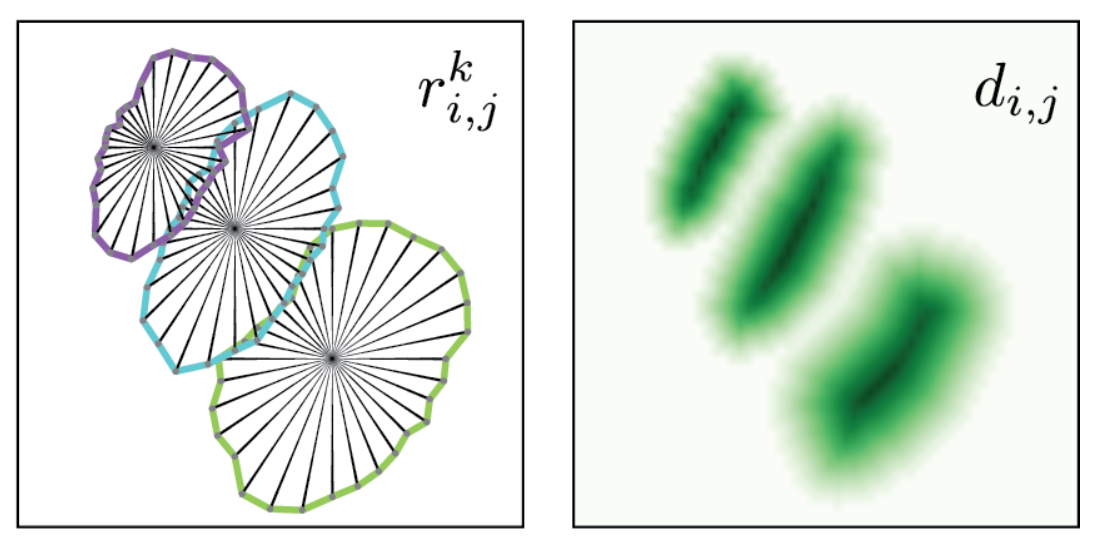
\includegraphics[width=8cm]{images/radialDistances.PNG}
    \caption{Radial Distances $r_{i,j}^{k}$ corresponding the euclidean distance to the boundary of each object by following one of the fixed angles. Object probabilities $d_{i,j}$ corresponding to the probability of presence of an object using Distance transform}
    \label{fig:radial}
    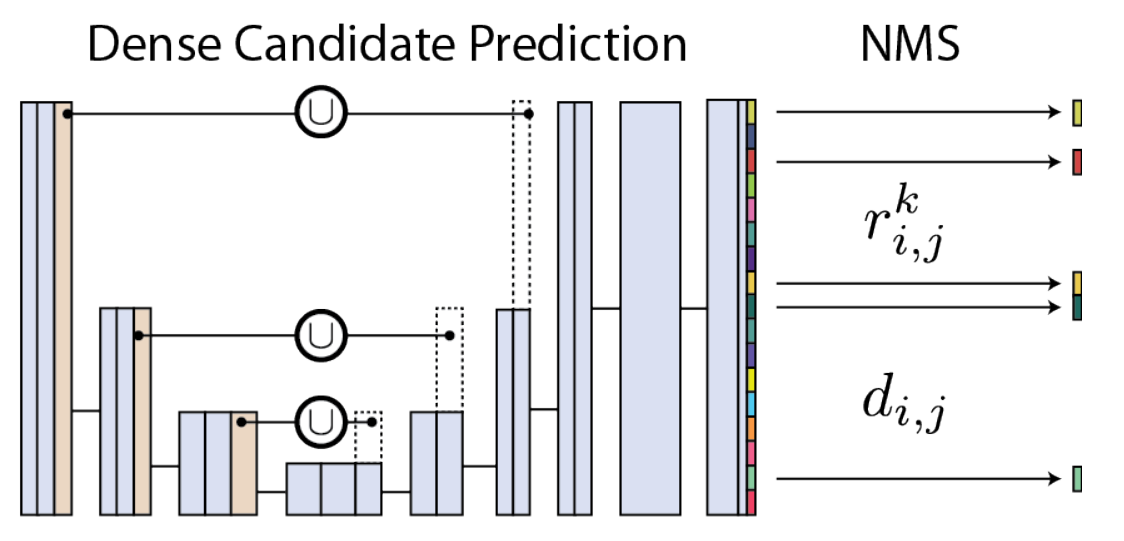
\includegraphics[width=8cm]{images/UnetStarDist.PNG}
    \caption{Stardist UNet model, where we pride ct for each pixel a set of 32 Radial Distances, and a object probability}

    \end{multicols}

    \label{fig:ac}
\end{figure}

\begin{equation}
    \mathcal{L}_{\mathit{StarDist}}(p_{ij}, \hat{p}_{ij}, R_{ij}, \hat{R}_{ij}) = \mathcal{L}_{\mathit{BCE}}(p_{ij}, \hat{p}_{ij}) + \lambda_1\mathcal{L}_{\mathit{radii}}(R_{ij}, \hat{R}_{ij}) 
    \label{eq:loss}
\end{equation}\\
Where $p_{ij}$ is the ground truth probability of object, $\hat{p}_{ij}$  is the predicted probability. $\mathcal{L}_{\mathit{BEC}}$ is the binary cross entropy loss. $R_{ij}$ is the set of all the R radial distances $\{r_{ij}^{k}\}_{k=1 \dots R}$ , and $\hat{R}_{ij}$ is the set of predicted R distances. $\lambda_1$ is a regularization factor. $\mathcal{L}_{\mathit{radii}}$ is a mean absolute error loss weighted by the ground truth probabilities, expressed as :
\begin{equation}
    \mathcal{L}_{\mathit{radii}} = p_{ij}.1_{p_{ij}>0}.\frac{1}{R}\sum_{k=0}^{R-1}|r_{ij}^{k}-\hat{r}_{ij}^{k}| + \lambda_2.1_{p_{ij}=0}\sum_{k=0}^{R-1}|\hat{r}_{ij}^{k}|
    \label{eq:lossradii}
\end{equation}
Where $\lambda_2$ is a regularization factor.\\

This loss is averaged for all pixels :
\begin{equation}
    \mathcal{L}_{\mathit{StarDist}} = \frac{1}{NM}\sum_{i=0}^{N}\sum_{j=0}^{M}\mathcal{L}_{\mathit{StarDist}}(p_{ij}, \hat{p}_{ij}, R_{ij}, \hat{R}_{ij})
\end{equation}

\begin{figure}[H]
    \centering
    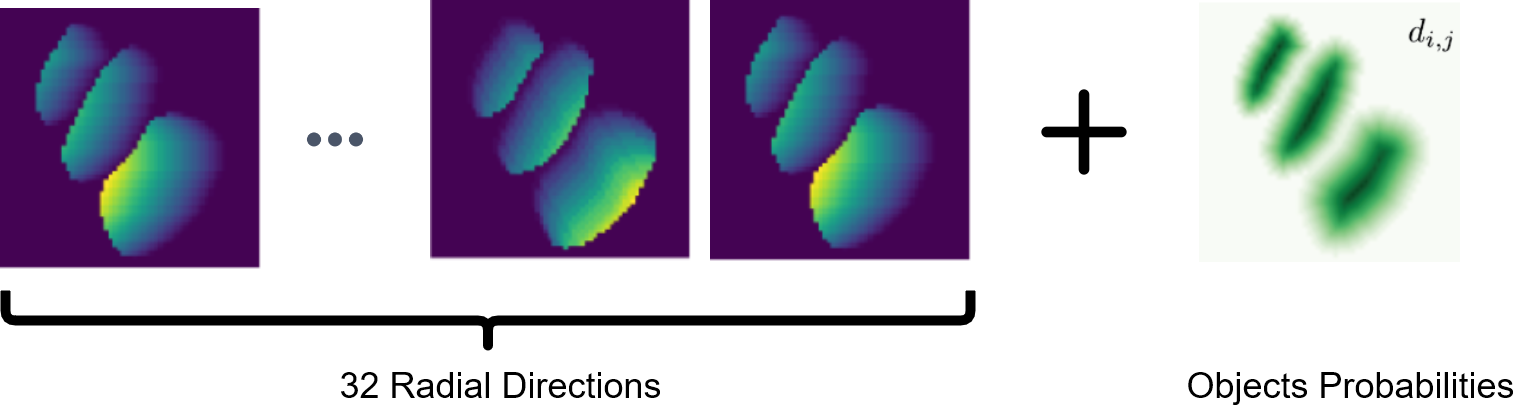
\includegraphics[width=16cm]{images/StardistPredictions.png}
    \caption{Stardist predicts densely a convex star polygon for each pixel, the output layer, correspond to 32 maps one for each radial direction where each pixel is the estimated distance to the object boundary by following the i-th radial direction, with objects probability for each pixel}
    \label{fig:stardistOutput}
\end{figure}

From the generated object probabilities and distances, we can sample polygons using the distribution P, but one problem emerge which is the multiple identification of the same object, to solve this , the author used a typical non maximum suppression (They keep the object with the highest probability, then compare it with the proposed polygons, if the intersection over union with that polygon is higher than some threshold then we consider that it's the same object detected twice and we keep only the most probably one, otherwise we consider that they represent two distinct object in that case we keep them both) (see \textbf{Figure \ref{fig:nms}}). 

\begin{figure}[H]
    \centering
    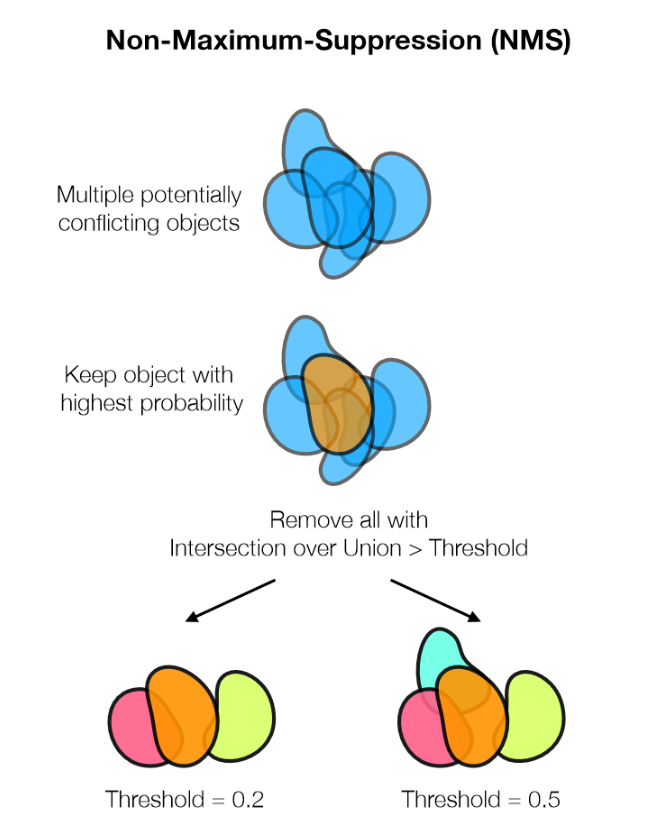
\includegraphics[width=8cm]{images/nms.png}
    \caption{From the potential polygons sampled from the object probabilities, a Non Maximum suppression is applied to remove duplicate detections}
    \label{fig:nms}
\end{figure}

In the time of evaluation, as used in older detection algorithms, we compute the true positives, false positives and false negatives, by matching the intersection over union of polygons predicted with ground truth polygons, for each object we match it with it's best (similar) match, then we apply a threshold to the intersection over union to control at what point a certain proposal is considered to be correct. (see \textbf{Figure \ref{fig:stardistOutput}})

\begin{figure}[H]
    \centering
    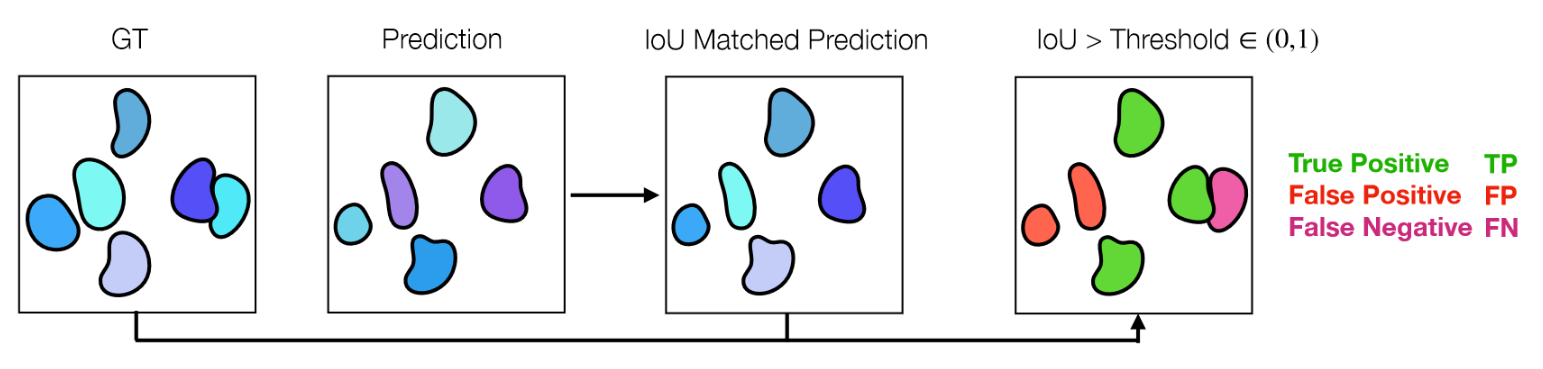
\includegraphics[width=16cm]{images/stardistEval.PNG}
    \caption{Stardist evaluation of predictions}
    \label{fig:stardistOutput}
\end{figure}

\subsection{Multistar}
In ~\cite{Walter2020}, the authors propose an extension of StarDist. They first show that using basic non maximal suppression is not optimal in the case of overlapping cells. They predict object overlap probability in addition to object presence and radial distances. They utilize this probability to improve proposal sampling while avoiding suppressing proposals of actually overlapping objects. This enables us to apply the concepts of StarDist to images with overlapping objects while introducing just a minimal overhead. 

\begin{figure}[H]
    \centering
    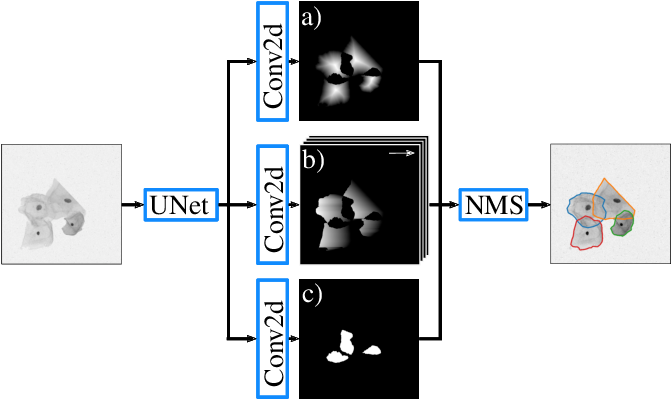
\includegraphics[width=8cm]{images/multistar.png}
    \caption{Multistar model}
    \label{fig:ac}
\end{figure}
\subsection{SplineDist}
Recent method ~\cite{Mandal2020} propose a further improvement to StarDist. they identify that the starconvexity constraint is very limiting as cells often have non starconvex shape (see \textbf{Figure \ref{fig:starxonvex}}). they choose to model the objects with B-Splines which requires way less control points and achieve more accurate shapes (see \textbf{Figure \ref{fig:splineangles}}).

\begin{figure}[H]
    \centering
    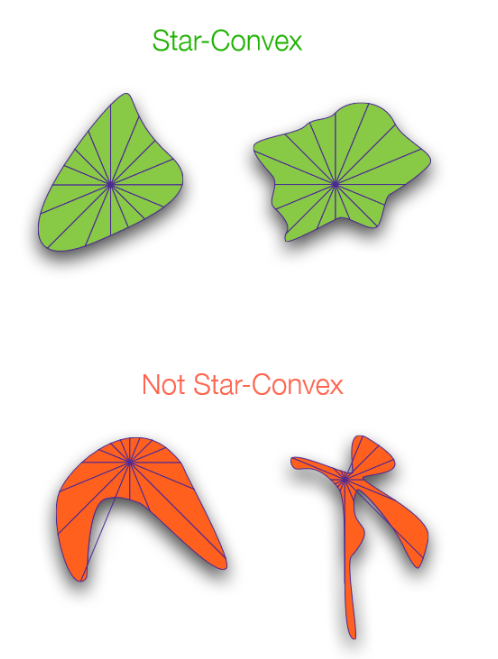
\includegraphics[width=4cm]{images/starconvex.png}
    \caption{Difference between star convex and non starconvex shapes}
    \label{fig:starxonvex}
\end{figure}

\begin{figure}[H]
    \centering
    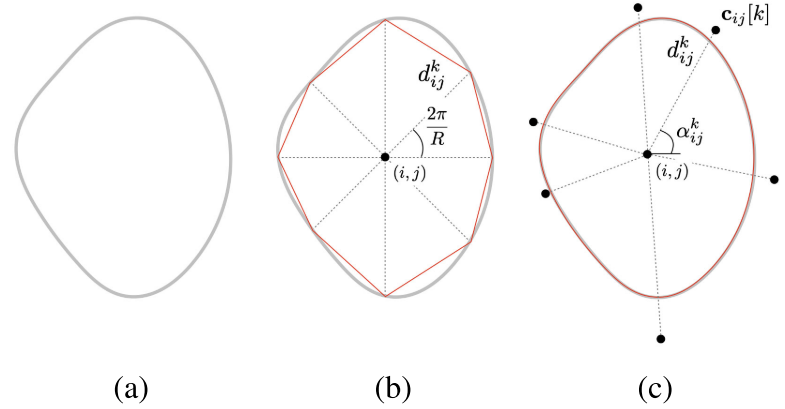
\includegraphics[width=8cm]{images/splinevsstarangles.png}
    \caption{SplineDist representation compared to StarDist}
    \label{fig:splineangles}
\end{figure}

The Model works as follows. we take a Unet very similar to the one proposed by StarDist. Now instead of predicting R radial distances, SplineDist predicts M pairs corresponding to control points (the first element, is the distance $d_{ij}^{k}$, the second correspond to an angle $\alpha_{ij}^{k}$) for each pixel of the image .This two values constitute the control point $c_{ij}[k]$. the final spline can be computed using :

\begin{equation}
    s(t) = \left[ \begin{matrix}
        s_x(t)\\
        s_y(t)
    \end{matrix}\right] = \sum_{k=0}^{M-1} c[k]\mathcal{\phi}_M(t-k) 
\end{equation}
where $\phi_M(t) = \sum_{m \in \mathbb{Z}}{\phi(t - Mm)}$ is the periodized version of a predefined spline basis $\phi$\\


For the evaluation, we apply a similar Non maximum suppression used in stardist for the proposed objects to keep only relevant ones, followed by a matching step, then as there is no ground truth value of the position of the control point (They can be anywhere, and sometimes different set of control point achieve the same exact curve), the authors choose to discretize the spline  (see \textbf{Figure \ref{fig:gtcontour}}) and compare the predicted contour to the ground truth one (obtained using Satoshi approach of border following ~\cite{Suzuki1985})
\begin{figure}[H]
    \centering
    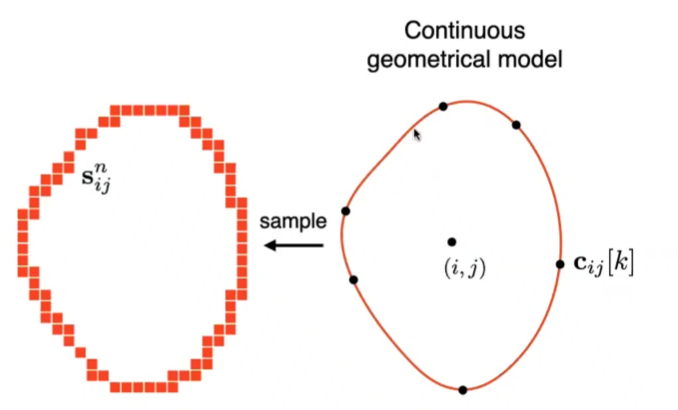
\includegraphics[width=8cm]{images/splinedistEval.PNG}
    \caption{Spline dist evaluation}
    \label{fig:gtcontour}
\end{figure}

The loss used is very similar to \textbf{Eq \ref{eq:loss}}:

\begin{equation}
    \mathcal{L}_{\mathit{StarDist}}(p_{ij}, \hat{p}_{ij}, P_{ij}, S_{ij}) = \mathcal{L}_{\mathit{BCE}}(p_{ij}, \hat{p}_{ij}) + \lambda_1\mathcal{L}_{\mathit{contour}}(P_{ij}, S_{ij}) 
\end{equation}
where $P_{ij}$, is the ground truth contour, $S_{ij}$ is the discretized predicted contour.\\

The contour loss $\mathcal{L}_{\mathit{contour}}$ simillarly to (\textbf{Eq \ref{eq:lossradii}}) is given by :

\begin{equation}
        \mathcal{L}_{\mathit{radii}}(p_{ij}, P_{ij}, S_{ij}) = p_{ij}.1_{p_{ij}>0}.\frac{1}{N}\sum_{n=0}^{N-1}|P_{ij}^{n}-S_{ij}^{n}| + \lambda_2.1_{p_{ij}=0}\sum_{n=0}^{N-1}|S_{ij}^{n}|
\end{equation}


\end{document}

